\providecommand{\topdir}{..}
\documentclass[\topdir/main.tex]{subfiles}

%External sources
\graphicspath{{\topdir/img/A01/}}

\begin{document}
\section{Introduction}
Bézier curves are a type of parametric curves invented by Pierre Bézier in the 1960s. They are widely used in graphic design software and \gls{cad} tools, as they provide an intuitive control over the shape of the curve. This intuitiveness is achieved using control points, which in colloquial terms, attract the curve towards them. The number of control points that are used define the degree of the curve\cite{pomax:bezier}. Nowadays, most programs use cubic Bézier curves, which are defined by 2 control points plus the two extreme points, as shown in the figure \ref{fig:cubic}.\newline

\begin{figure}[hbtp]
    \centering
    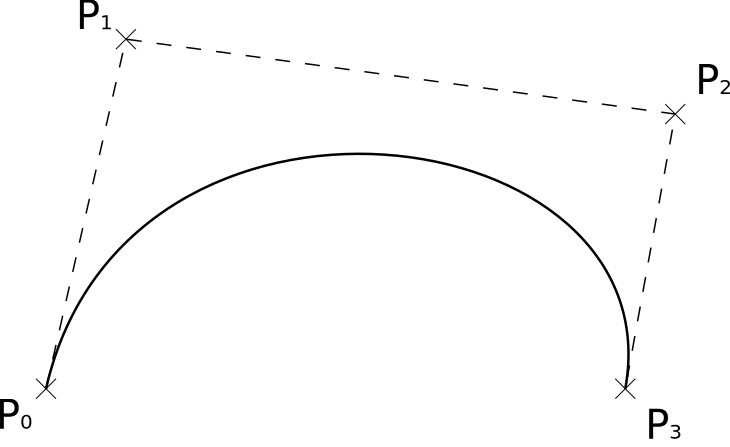
\includegraphics[width=0.5\textwidth]{Cubic Bezier curve}
 
    \caption{Cubic Bézier example}
    \label{fig:cubic}
\end{figure}

Modern \glspl{gpu} are highly specialized in rendering triangles. Therefore, it may seem that rendering smooth Bézier curves is an impossible task for this hardware. However, in the last 2 decades, several approaches have been developed to solve this problem.\newline

Some of them rely on segmenting the curves in very short lines, so that it appears to be quasi-smooth. This approach involves creating lots of vertices and thin triangles, which might hurt performance and memory availability. Moreover, unless external anti-aliasing is used, the edges will appear to be jaggy.\newline

Some other approaches are based on uploading the contour data to the \gls{gpu} and processing it in a fancy fragment shader. They usually feature a \gls{sdf} based anti-aliasing mechanism, so the edges appear to be smooth. However, for the sake of optimization, they might not obtain pixel-perfect results, while having a very heavy impact on the performance, as the curves need to be processed once per frame. This may make them a good candidate for mutating curves, but do not suit more static scenarios.\newline

Here is where Loop-Blinn's solution comes into place. This solution consists in describing the Bézier curve as a set of implicit curve equations and assigning its value to each of the rendered pixels\cite{loopblinn2005}. This approach is highly efficient due to its linearity, although it requires a bit of preliminary \textit{number crunching} in the \gls{cpu}.\newline %TODO explain better

This last approach has been chosen to crop video frames with an arbitrary shape. In particular, cubic curves will be used, as they have become an industry standard.

\section{Mathematical definition of Bézier curves}
The analytical form of the Bézier curves is based on polynomials of arbitrary degree. For a $N$-degree Bézier curve, $N+1$ control points are needed, where two of them will be the start and end points. Therefore, a cubic curve is defined by 4 control points, as shown in the figure \ref{fig:cubic}. The generic form for a $N$-degree Bézier curve is displayed in the equation \eqref{eq:bezier} \cite{pomax:bezier, wiki:bezier}. Setting $N=3$ for cubic curves, the equation \eqref{eq:bezier3} is obtained.\newline

\begin{equation} \label{eq:bezier}
    B(t) = \sum_{i = 0}^{N} P_i \cdot b_{N,i}(t) \qquad t \in [0, 1]
\end{equation}

where $b_{N,i}$ is the $N$-th degree Bernstein basis polynomial's $i$-th term, which is defined as \eqref{eq:bernstein}.\newline

\begin{equation} \label{eq:bernstein}
    b_{N,i}(t) = \binom{N}{i} (1-t)^{N-i} t^i \qquad t \in [0, 1]
\end{equation}

\begin{equation} \label{eq:bezier3}
    B_3(t) = P_0(1-t)^3 + 3P_1(1-t)^2t + 3P_2(1-t)t^2 + P_3t^3 \qquad t \in [0, 1]
\end{equation}

Multiple Bézier curves can be chained one after the other so that the end-point of one curve is the beginning of the next one. This is commonly known as a polycurve. If both ends of the curve meet, a closed contour is formed. These closed contours will be the input data for the algorithm.\newline 

Any Bézier curve can be expressed in terms of a higher order curve, although the reverse operation is not generally possible. For instance, cubic curves can be used to draw quadratic curves or lines, as lines can be thought of as first degree curves \cite{pomax:bezier}. This property will become handy in later stages where the implementation of the algorithm is described. Moreover, a Bézier curve can be subdivided in many shorter segments of same degree.\newline

The derivative of a Bézier curve will be another Bézier curve of one degree lower. As all terms are multiplied by $t^N$, $N$ must be multiplied by the derivative, due to the polynomial derivation rules. The new control points will be the differences between consecutive pairs of points in the original curve, as displayed in the equation \eqref{eq:bezier_dt}.

\begin{equation} \label{eq:bezier_dt}
    \frac{d}{dt} B(t) = N \sum_{i = 0}^{N-1} (P_{i+1} - P_i) \cdot b_{N-1,i} \qquad t \in [0, 1]
\end{equation}

If $t=0$ and $t=1$ are substituted in the expression \eqref{eq:bezier}, the equation simplifies down to $P_0$ and $P_N$ respectively, this is, the extreme points of the curve. If the same values are substituted in the derivative, the expression is simplified to the difference between the extreme points and its neighbor. These four trivial cases are displayed in the equation \eqref{eq:bezier_trivial}. Although they might seem useless at first glance, they play a key role on the intuitiveness of the Bézier curves. It can be easily inferred that the curve in the extreme points will be tangent to the line joining the extreme point with its neighboring control point. This can be confirmed observing the figure \ref{fig:cubic}, where the curve in $P_0$ is tangent to $\overrightarrow{P_0P_1}$ and tangent to $\overrightarrow{P_2P_3}$ in $P_3$.\newline

\begin{equation} \label{eq:bezier_trivial}
    B(0) = P_0 \quad B(1) = P_N \quad \frac{d}{dt} B(0) = N(P_1 - P_0) \quad \frac{d}{dt} B(1) = N(P_{N-1} - P_N)
\end{equation}

This statement has also an impact on the polycurves. A polycurve will only be derivable at the transition point between the segments if the following condition is met: The penultimate control point of a segment must lie on the line joining the first and second control points of the next segment -remember that due to continuity, the first control point of the next segment is also the last control point of the current segment-. This derivability condition is known as C1 continuity. Although it does not have to be met, it does have an artistic meaning: The absence or presence of corners.

\section{Loop Blinn's algorithm implementation}
Loop Blinn's Bézier curve rasterization algorithm was developed by Charles Loop and Jim Blinn in 2005. For the purposes of this project, a variant of this algorithm has been implemented to be able to crop a video frame with an arbitrary shape. The original algorithm has two variants, the first one being for quadratic curves and the other one for cubic curves. In this case, the later one has been chosen, as quadratic curves can be easily converted into cubic curves.

\subsection{The test image}
This algorithm must handle some extreme cases. Therefore, to showcase how all those situations are handled, the test image must feature them. For this reason, the vectorization of a whale shown in the figure \ref{fig:whale} has been chosen, as it provides the following special cases:

\begin{itemize}
    \item No holes, as currently they are not supported.
    \item Multiple independent contours. In this test image, 4 bodies can be distinguished: The whale itself and 3 drops of water.
    \item Highly convex shape.
    \item Star-like sections: The tail forms a 3 tipped star.
    \item Straight lines, which can be spotted in the root of the center droplet.
    \item Quadratic curves
    \item S shaped cubic curves, which form the whale's tail fins.
    \item U shaped cubic curves, which are the most common ones.
    \item Curves that come very close, as it does on the tail.
\end{itemize}

\begin{figure}[hbtp]
    \centering
    \subfigure[Filled]{\includegraphics[width=0.45\textwidth]{Whale Fill}}
    \subfigure[Outline with control points]{\includegraphics[width=0.45\textwidth]{Whale Ctrl}}

    \caption{Vectorization of a cartoon whale}
    \label{fig:whale}
\end{figure}

\subsection{Procedure}
As mentioned before, the input data for the algorithm is a collection of contours which in turn are formed by multiple cubic Bézier curves. As the contour must be continuous and closed, two consecutive segments share a single extreme point, so there is no need to store it twice. Therefore, for a given contour formed by $M$ $N$-degree segments, $M \cdot N$ points will be used to store the contour. Note that each of the individual segments is defined by $N+1$ control points.\newline 

Although the algorithm aims to have as few as possible input restrictions, there is one condition that the input must meet: The contours must not self-intersect. An example of a valid and invalid contour is displayed in the figure \ref{fig:valid}\newline

\begin{figure}[hbtp]
    \centering
    \subfigure[Valid]{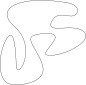
\includegraphics[width=0.45\textwidth]{Valid Contour}}
    \subfigure[Invalid]{\includegraphics[width=0.45\textwidth]{Invalid Contour}}

    \caption{Valid and invalid input data}
    \label{fig:valid}
\end{figure}

Most of the operations described in the following steps will be performed repeatedly on each of the contours. Therefore, only the body of the whale will be used as an example for those steps.\newline

\subsubsection{Contour sanitation}
In the context of computer graphics, contours and polygons are usually described in \gls{ccw} order. In fact, if a contour is defined as \gls{cw}, it is usually to signal that it is a hole inside another bigger contour. This convention is illustrated in the figure \ref{fig:winding}. However, as mentioned earlier, this algorithm does not currently support holes, so all \gls{cw} contours are turned into \gls{ccw} by reversing the order of its points. Therefore, from now on, all contours can be assumed to be \gls{ccw}.\newline

\begin{figure}[hbtp]
    \centering
    
\includegraphics[width=0.7\textwidth]{Winding}

    \caption{Winding convention}
    \label{fig:winding}
\end{figure}


\subsubsection{Outer-hull triangulation}
As mentioned before, cubic segments are defined by four control points. Due to the curve tangency properties, which were described earlier, it can be ensured that a cubic Bézier curve will not escape the convex polygon formed by its four control points. This is a strong property, as all calculations can be narrowed down to this area. As these computations will be performed in the fragment shader of the \gls{gpu}'s graphics pipeline, this convex polygon needs to be triangulated. The collection of convex polygons regarding each of the segments, will be called the outer hull. Each of the pixels rastered by the outer hull will have to be individually evaluated to determine whether it is inside or outside the contour.\newline 

Note that until this point the term \textquote{convex polygon} has been vaguely used. This is because the nature of it is unknown. Therefore, the first step is to determine the convex shape formed by the control points. This can be boiled down to two cases, assuming that the control points are not colinear nor the same point. The first case is the trivial one, the four points form a convex quadrilateral. The other one is the tricky case, which occurs when they form a concave quadrilateral, as shown in the figure \ref{fig:quad_triang}. In this situation, a triangle -which is always convex- will be formed, containing one of the points inside.\newline

\begin{figure}[hbtp]
    \centering
    \subfigure[Convex quadrilateral]{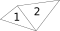
\includegraphics[width=0.3\textwidth]{Convex Quad triangulation}}
    \subfigure[Concave quadrilateral turned into a triangle]{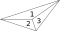
\includegraphics[width=0.3\textwidth]{Concave Quad triangulation}}

    \caption{Triangulation of the outer-hull}
    \label{fig:quad_triang}
\end{figure}

In the first case, the triangulation is performed by splitting the quad on its shortest diagonal. The benefit of splitting it on its shortest diagonal is that repeated pixel calculations are minimized. In the second case, three triangles will be formed, all having the middle vertex in common. For the sake of avoiding repeated vertex shader executions, both triangulations are made in a triangle-strip compatible manner and using a index buffer. This adds extra complexity to the algorithm, but it may be beneficial for complex contours.\newline

If two curves come very close, their bounding convex polygons may collide. This can lead to rendering artifacts, so it needs to be addressed. The solution adopted here is fairly crude, as this is not a common case. The solution consists of splitting both colliding segments in halves, using the method described earlier. All cases that occur on the whale's image have been highlighted in the figure \ref{fig:whale_intersections}. There is another potential case that requires splitting a segment in two. This other situation will be mentioned later.\newline

\begin{figure}[hbtp]
    \centering
    \subfigure[Intersections]{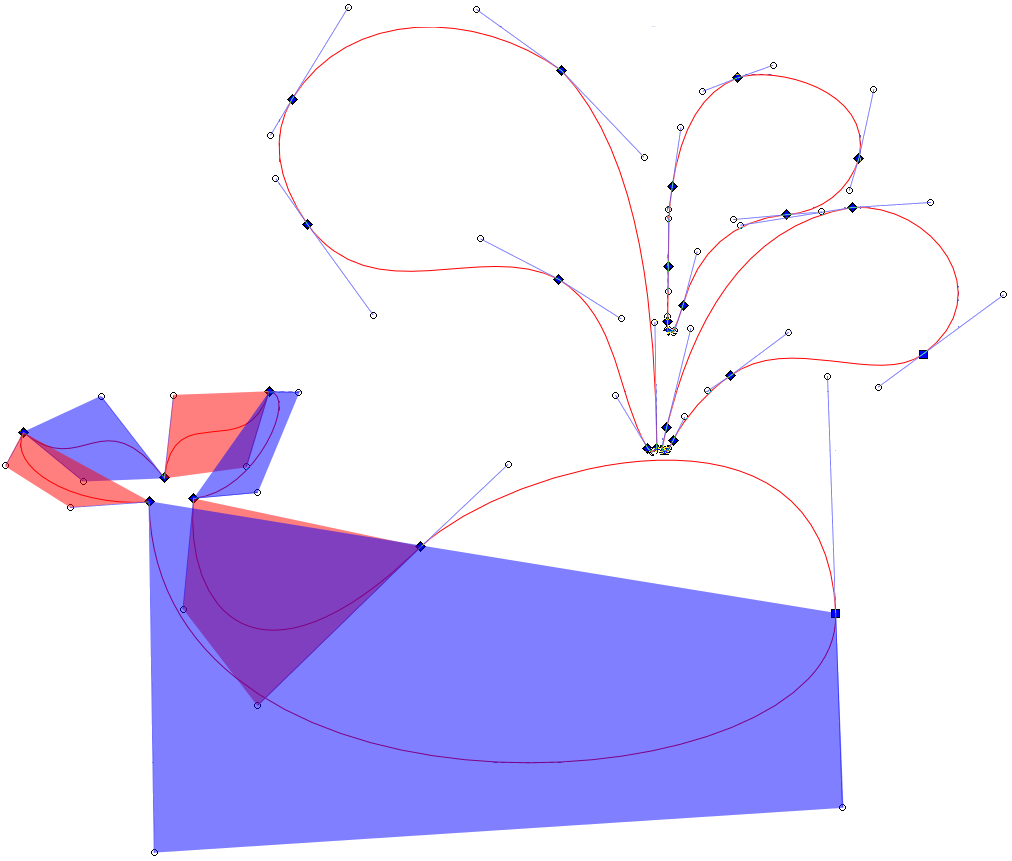
\includegraphics[width=0.45\textwidth]{Whale Ctrl Intersections}}
    \subfigure[After splitting]{\includegraphics[width=0.45\textwidth]{Whale Ctrl}}

    \caption{Vectorization of a cartoon whale}
    \label{fig:whale_intersections}
\end{figure}

\subsubsection{Inner-hull extraction and triangulation}
After defining the outer hull, a big unfilled void remains in the middle of the contour. Luckily, it can be ensured that this arbitrarily shaped polygon is fully inside the contour. Therefore, the only task regarding it is to triangulate. The algorithm selected for this task is based on the source code of PolyPartition\cite{polypartition}, although it has been optimized to avoid unnecessary calculations and heap allocations.\newline

The first step is to determine which pairs of vertices are mutually visible. Assuming that the polygon does not self-intersect, it can be ensured that consecutive points are mutually visible. However, this may not be true for other pairs of vertices if the polygon is concave. For the sake of testing their visibility, the intersection between the line joining them and all edges of the polygon is computed. Moreover, this line must lie between the two edges associated with the departing vertex. If no intersection is found and the line does not exit the polygon, it can be considered a diagonal. In the figure \ref{} several examples of these conditions are displayed.\newline

The only remaining step is to choose the appropriate diagonals to triangulate the polygon. To begin with, a random edge of the polygon is placed into a queue, which was previously empty. Then, a line is extracted from this queue -obviously, the first time, this line will be the newly placed edge-. For this line, the closest vertex to which diagonals or edges can be traced is chosen. These diagonals -not the edges- are pushed into the queue, so that they are the starting point for future iterations. This process is repeated indefinitely until the queue is empty. On each iteration, zero, one, or two diagonals will be added to the queue, while a single one will be removed. A possible execution is shown in the figure \ref{}.\newline

The only reason for not supporting holes is that the chosen triangulation algorithm does not support them. Its not even an efficient algorithm, as it has $O(n^3)$ complexity, but it provides the best triangulation in all situations. Definitively, there is a lot of room for improvement in this section. Therefore, for future releases, a Constrained Delaunay triangulation algorithm will be considered. This is the algorithm used by Charles Loop and Jim Blinn in their paper\cite{loopblinn2005}. This other algorithm has $O(n \log n)$ complexity\cite{wiki:constrained_delaunay}.\newline

\subsubsection{Homogeneous implicit line coordinate calculation}
Until this point, C. Loop and J. Blinn's algorithm has been followed \textit{a grosso modo}, adding the author's own criteria. However, this part of the algorithm has been implemented as a mere copy of the equations described in their article\cite{loopblinn2005} and their chapter in GPU Gems 3\cite{GPUGems3C26}. As a recap, until this point, we have separated a cubic Bézier contour in two parts. The first one, the outer hull, corresponds to the parts of the shape that are going to be conditionally filled. The other one, the inner hull, will be fully filled. Therefore, the next logical step is to implement a method to determine which pixels of the outer hull correspond to the inside of the contour and which ones to the outside, as only the ones that are inside will have to be filled.\newline

As stated by C. Loop and J. Blinn, \textquote{A simple implicit equation for a parametric curve is found in a space that can be thought of as an analog to texture space}\cite{loopblinn2005}. This means that any Bézier curve can be mapped to those implicit equations which will be linearly interpolated. Therefore, the main goal of this section is to calculate the implicit equations that belong to each of the control points.\newline

This implicit equation will be \eqref{eq:bezier_blinnloop3} for cubic curves. Luckily, $n$ always equals to $1$ as the line that it represents is always at infinity. Therefore, the actual equation will be \eqref{eq:bezier_blinnloop3_2}. This implies that a $[k, l, m]$ vector will have to be assigned to each of the control points in order to map the $c(x, y)$ implicit function to space.

\begin{equation} \label{eq:bezier_blinnloop3}
    c(x, y) = k^3 - lmn
\end{equation}

\begin{equation} \label{eq:bezier_blinnloop3_2}
    c(x, y) = k^3 - lm
\end{equation}



The input for this section will be each of the individual segments that form the outer hull. According to Jim Blinn's Corner\cite{blinn2002}, a cubic segment can be classified as one of the following topologies:

\begin{itemize}
    \item Serpentine
    \item Loop
    \item Cusp: The transition point between serpentine and loop
    \item Quadratic
    \item Line
    \item Point
\end{itemize}

As the equations vary from topology to topology, the first step is to classify the segment. For this task the $\delta_1, \delta_2, \delta_3$ parameters and the discriminant are calculated according to the equations \eqref{eq:loopblinna} \eqref{eq:loopblinnd} \eqref{eq:loopblinndisc}. Note that a affine space is used, so that $P_i' = [P_i, 1]$. This is how the mixed product of 2D points is defined. As a small caveat, the result of the mixed product may get very large, easily overwhelming 32bit float-s. Luckily, multiplying the result by a constant does not alter the outcome, so the $a$ values should be normalized to avoid computing the $\delta$-s with large numbers, potentially introducing floating-point errors.

\begin{equation} \label{eq:loopblinna}
    a_1 = P_0 \cdot P_3 \times P_2 \qquad
    a_2 = P_1 \cdot P_0 \times P_3 \qquad
    a_3 = P_2 \cdot P_1 \times P_0
\end{equation}

\begin{equation} \label{eq:loopblinnd}
    \delta_1 = a_1 - 2a_2 + 3a_3 \qquad
    \delta_2 = -a_2 - 3a_3 \qquad
    \delta_3 = 3a_3
\end{equation}

\begin{equation} \label{eq:loopblinndisc}
    disc = \delta_1^2 \cdot (3\delta_2^2 - 4\delta_1\delta_3)
\end{equation}

The next step is to obtain the homogeneous implicit line coordinates according to the curve's topology. Each of the topologies is characterized by a particular set of conditions regarding the $\delta$ values and the discriminant. The $P_i$ control point's $klm$ vector will be denoted as $F_i$:

\begin{itemize}
    \item \textbf{Line or point}: $\delta_1 = 0, \delta_2 = 0, \delta_3 = 0$\\
        As lines and points can be considered 1D or 0D, they do not form an area to fill, so they can be simply discarded. 
    
    \item \textbf{Quadratic}: $\delta_1 = 0, \delta_2 = 0, \delta_3 \neq 0$\\
        \begin{table}[H]
            \centering
            \begin{tabular}{|l|c|c|c|}
                \hline
                \qquad&     $k$ &               $l$ &               $m$             \\\hline
                $F_0$ &     $0$ &               $0$ &               $0$             \\\hline
                $F_1$ &     $\sfrac{1}{3}$ &    $0$ &               $\sfrac{1}{3}$  \\\hline
                $F_1$ &     $\sfrac{2}{3}$ &    $\sfrac{1}{3}$ &    $\sfrac{2}{3}$  \\\hline
                $F_0$ &     $1$ &               $1$ &               $1$             \\\hline
            \end{tabular}
            \caption{Homogeneous implicit line equation coefficients for quadratic curves}
            \label{tab:blinnloop_klm_quadratic}
        \end{table}
    
    \item \textbf{Serpentine}: $\delta_1 \neq 0, \delta_2 \neq 0, disc > 0$
        \begin{table}[H]
            \centering
            \begin{tabular}{|l|c|c|c|}
                \hline
                \qquad&     $k$ &               $l$ &               $m$ \\\hline
                $F_0$ &     $l_s m_s$ &         $l_s^3$ &           $m_s^3$ \\\hline
                $F_1$ &     $l_s m_s - \sfrac{1}{3} l_s m_t - \sfrac{1}{3} l_t m_s$ &       
                            $l_s^2 (l_s - l_t)$ &         
                            $m_s^2 (m_s - m_t)$ \\\hline
                $F_2$ &     $l_s m_s - \sfrac{2}{3} l_s m_t - \sfrac{2}{3} l_t m_s - \sfrac{1}{3} l_t m_t$ &
                            $l_s (l_s - l_t)^2$ &
                            $m_s (m_s - m_t)^2$ \\\hline
                $F_3$ &     $(l_s - l_t) (m_s - m_t)$ &  
                            $(l_s - l_t)^3$ &  
                            $(m_s - m_t)^3$ \\\hline
            \end{tabular}
            \caption{Homogeneous implicit line equation coefficients for serpentines}
            \label{tab:blinnloop_klm_serpentine}
        \end{table}
        
        where $l_s$, $l_t$, $m_s$ and $m_t$ are obtained as displayed in the equation \eqref{eq:blinnloop_klm_serpentine_lm}
        
        \begin{equation} \label{eq:blinnloop_klm_serpentine_lm}
            l_s = 3\delta_2 - \sqrt{3(3\delta_2^2 - 4\delta_1\delta_3)} \qquad
            m_s = 3\delta_2 + \sqrt{3(3\delta_2^2 - 4\delta_1\delta_3)} \qquad
            l_t = m_t = 6 \delta_1
        \end{equation}

     
    \item \textbf{Cusp}: $\delta_2 \neq 0, disc = 0$
        \begin{table}[H]
            \centering
            \begin{tabular}{|l|c|c|c|}
                \hline
                \qquad&     $k$ &               $l$ &               $m$             \\\hline
                $F_0$ &     $l_s$ &             $l_s^3$ &           $1$             \\\hline
                $F_1$ &     $l_s - \sfrac{1}{3} l_t$ &    
                            $l_s^2 (l_s - l_t)$ &               
                            $1$ \\\hline
                $F_2$ &     $l_s - \sfrac{2}{3} l_t$ &    
                            $l_s (l_s - l_t)^2$ &               
                            $1$ \\\hline
                $F_0$ &     $(l_s - l_t)$ &     $(l_s - l_t)^3$ &   $1$             \\\hline
            \end{tabular}
            \caption{Homogeneous implicit line equation coefficients for cusps}
            \label{tab:blinnloop_klm_cusp}
        \end{table}
        
        where $l_s$, and $l_t$  are obtained as displayed in the equation \eqref{eq:blinnloop_klm_cusp_lm}
    
        \begin{equation} \label{eq:blinnloop_klm_cusp_lm}
            l_s = \delta_3\qquad
            l_t = 2 \delta_1
        \end{equation}
    
    
    \item \textbf{Loop}: $\delta_1 \neq 0, \delta_2 \neq 0, disc < 0$
        \begin{table}[H]
            \centering
            \scriptsize
            \begin{tabular}{|l|c|c|c|}
                \hline
                \qquad&           $k$ &               $l$ &               $m$ \\\hline
                $F_0$ &     $l_s m_s$ &         $l_s^2 m_s$ &       $l_s m_s^2 $ \\\hline
                $F_1$ &     $l_s m_s - \sfrac{1}{3} l_s m_t - \sfrac{1}{3} l_t m_s$ &       
                            $l_s^2 m_s - \sfrac{2}{3} l_s l_t  m_s - \sfrac{1}{3} l_s^2 m_t$ &         
                            $l_s m_s^2 - \sfrac{2}{3} l_s m_s m_t - \sfrac{1}{3} l_t m_s^2$ \\\hline
                $F_2$ &     $l_s m_s - \sfrac{2}{3} l_s m_t - \sfrac{2}{3} l_t m_s - \sfrac{1}{3} l_t m_t$ &
                            $(l_s-l_t)(l_s m_s - \sfrac{2}{3} l_s m_t - \sfrac{1}{3} l_t m_s)$ &
                            $(m_s-m_t)(l_s m_s - \sfrac{2}{3} l_t m_s - \sfrac{1}{3} l_s m_t)$ \\\hline
                $F_3$ &     $(l_s - l_t) (m_s - m_t)$ &  
                            $(l_s - l_t)^2 (m_s - m_t)$ &  
                            $(l_s - l_t) (m_s - m_t)^2$ \\\hline
            \end{tabular}
            \caption{Homogeneous implicit line equation coefficients for loops}
            \label{tab:blinnloop_klm_loop}
        \end{table}
        
        where $l_s$, $l_t$, $m_s$ and $m_t$ are obtained as displayed in the equation \eqref{eq:blinnloop_klm_loop_lm}
        
        \begin{equation} \label{eq:blinnloop_klm_loop_lm}
            l_s = \delta_2 - \sqrt{4\delta_1\delta_3 - 3\delta_2^2} \qquad
            m_s = \delta_2 + \sqrt{4\delta_1\delta_3 - 3\delta_2^2} \qquad
            l_t = m_t = 2 \delta_1
        \end{equation}
    
\end{itemize}

Once these coordinates are assigned to the control point vertices, they are uploaded to the \gls{gpu}'s local memory. When a draw call is issued, their values will be linearly interpolated at the rasterization stage, supplying to each of the executions of the fragment shader its own set of $klm$ values. Then the fragment shader evaluates the equation \eqref{eq:bezier_blinnloop3_2}. If it turns out to be greater than zero, that particular pixel is outside the contour and it can be discarded.\newline

Similarly to as proposed by Antonio J. Rueda, Juan Ruiz de Miras, and Francisco R. Feito in their paper \cite{ruedaruizfeito2008}, many parts of this later part of the algorithm could be executed by the geometry shader of the \gls{gpu}, instead of doing so in the \gls{cpu}. However, this last optimization has not been considered as geometry shader support is not mandatory in Vulkan, so a fallback method that computes the $klm$ values in the \gls{cpu} should be still available, greatly increasing the complexity and reducing maintainability.\newline 

\subsubsection{Signed distance estimation}
Considering all previous steps, the purposes of this chapter are already achieved. However, as displayed in the figure \ref{}, the edges appear to be jaggy due to the aliasing effect. With the aim of solving this, a widespread practice is to obtain the signed distance to the curve, this is, the distance from a point to the closest point on the curve with a different sign depending on the side of the contour on which the point lies. The convention is to use positive values for the outside while using negative ones for the inside.\newline

The $c(x, y)$ function displayed earlier has this particular tendency in points close to the contour, but with a small caveat: Its rate of change is not known. In order to implement a \gls{sdf} based anti-aliasing strategy, the distance to the border in pixels must be known, so that subpixel distances are used to modulate the intensity of frontier pixels. This metric can be obtained dividing $c(x, y)$ by the length of its gradient, as shown in the equation \eqref{eq:blinnloop_sdf}. This works because the gradient is approximately square to the border of its proximities. As a consequence, the $||\nabla sd(x, y)|| \approx 1$, which is one of the requirements for the signed distance functions.\newline

\begin{equation} \label{eq:blinnloop_sdf}
    sd(x, y) \approx \frac{c(x, y)}{||\nabla c(x, y)||} = \frac{c(x, y)}{\sqrt{[\frac{\partial}{\partial x} c(x, y)]^2 + [\frac{\partial}{\partial y} c(x, y)]^2}}
\end{equation}
        
The gradient of the $c$ function can be easily obtained by applying the chain rule. This is displayed in the equation \eqref{eq:blinnloop_sdf_gra} using the Jacobian matrix.

\begin{equation} \label{eq:blinnloop_sdf_gra}
    \nabla c(x, y) = 
    \begin{bmatrix}
        \frac{\partial c(x, y)}{\partial x} \\
        \frac{\partial c(x, y)}{\partial y}
    \end{bmatrix}
    =
    \begin{bmatrix}
        \frac{\partial k}{\partial x} & \frac{\partial l}{\partial x} & \frac{\partial m}{\partial x} \\
        \frac{\partial k}{\partial y} & \frac{\partial l}{\partial y} & \frac{\partial y}{\partial x}
    \end{bmatrix}
    \cdot
    \begin{bmatrix}
        3 k^2 \\
        -m \\
        -l
    \end{bmatrix}
\end{equation}

Modern \glspl{gpu} can approximate partial derivatives, as their processors are based on 2x2 or 4x4 \gls{simd} architectures. This means that at any given time, a 2x2 -or 4x4- group of pixels is being concurrently processed, allowing comparisons among them. In \gls{glsl}, the functions to obtain partial derivatives are named as \texttt{dFdx} and \texttt{dFdy} for $\frac{\partial}{\partial x}F(x, y)$ and $\frac{\partial}{\partial y}F(x, y)$, respectively.\newline

\printbibliography

\end{document}
